\documentclass[tikz]{standalone}
\usetikzlibrary{positioning}
\begin{document}
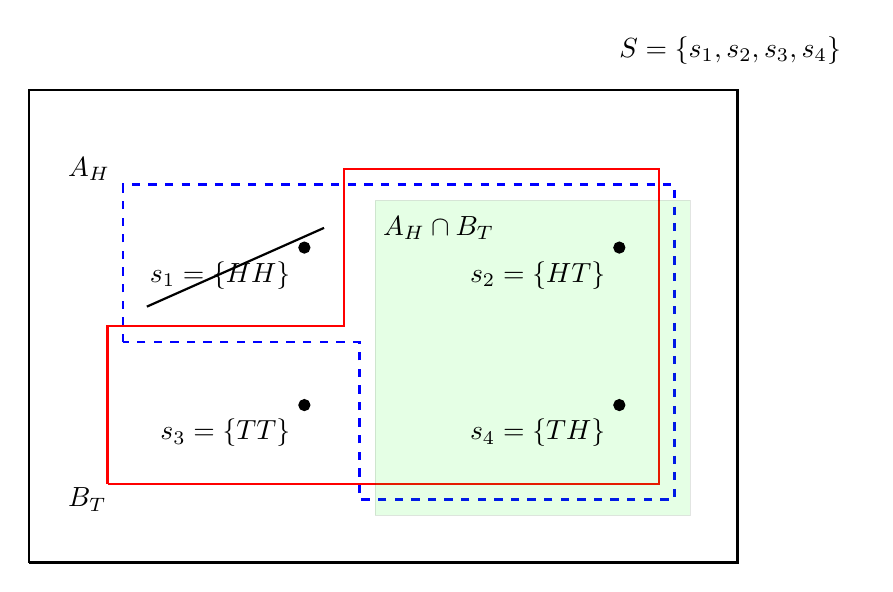
\begin{tikzpicture}[scale=1]
\draw[thick]
(0,0) coordinate --
(0,6) coordinate --
(9,6) coordinate --
(9,0) coordinate --
(0,0) coordinate;

\draw[thick,red]
(1,1) coordinate --
(1,3) coordinate --
(4,3) coordinate --
(4,5) coordinate --
(8,5) coordinate --
(8,1) coordinate --
(1,1) coordinate;

\begin{scope}[xshift=0.2cm,yshift=-0.2cm]
\draw[thick,dashed,blue]
(1,3) coordinate --
(1,5) coordinate --
(8,5) coordinate --
(8,1) coordinate --
(4,1) coordinate --
(4,3) coordinate --
(1,3) coordinate;
\end{scope}

\draw[thick]
(1.5,3.25) coordinate --
(3.75,4.25) coordinate;

\begin{scope}[xshift=0.4cm,yshift=-0.4cm]
\filldraw[fill=green,opacity=0.1]
(8,5) coordinate --
(8,1) coordinate --
(4,1) coordinate --
(4,5) coordinate --
(8,5) coordinate;
\end{scope}

\node[label=below left:{$s_1=\{HH\}$},draw,fill=black,circle,inner sep=0pt,minimum size=4pt] at (3.5,4) {};
\node[label=below left:{$s_2=\{HT\}$},draw,fill=black,circle,inner sep=0pt,minimum size=4pt] at (7.5,4) {};
\node[label=below left:{$s_3=\{TT\}$},draw,fill=black,circle,inner sep=0pt,minimum size=4pt] at (3.5,2) {};
\node[label=below left:{$s_4=\{TH\}$},draw,fill=black,circle,inner sep=0pt,minimum size=4pt] at (7.5,2) {};

\node[text width=3cm] at (9,6.5) {$S = \{s_1,s_2,s_3,s_4\}$};
\node[text width=1cm] at (1,5) {$A_H$};
\begin{scope}[yshift=-0.2cm]
\node[text width=1cm] at (1,1) {$B_T$};
\end{scope}
\node[text width=2cm] at (5.5,4.25) {$A_H \cap B_T$};

\end{tikzpicture}
\end{document}